\chapter{Unit of Work}

\section{Descrizione}

"Maintains a list of objects affected by a business transaction and coordinates the writing out of changes and the resolution of concurrency problems" - Martin Fowler

Quando si hanno dei dati che devono venire prograssivamente aggiornati in piu' parti di un applicativo ed e' importante tenere traccia di tutte le modifiche, assicurarsi che avvengano ciascuna correttamente senza conflitti dettati dalla concorrenza, e' possibile delegare le operazioni ad un unico soggetto che si occupi di gestire l'aggiornamento del sistema in modo sicuro ed efficiente.

\section{Vista UML}

\begin{center}
    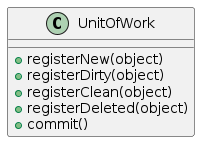
\includegraphics[width=6cm]{images/unit-of-work/UnitOfWorkClass.png}
    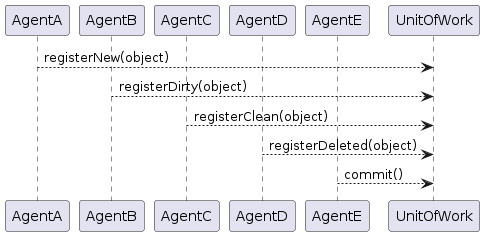
\includegraphics[width=12cm]{images/unit-of-work/UnitOfWorkSD.png}
\end{center}

\section{Vantaggi}

Centralizzare il meccanismo di aggiornamento dei dati permette di sfruttare in modo piu' efficiente le operazioni onerose, come le interazioni con il Database. Invece di avere tante piccole chiamate di scrittura su Database si puo' averne poche, o una sola, piu' pesanti. Apparentemente potrebbe sembrare una peggior soluzione, tuttavia molti, se non tutti, Database consentono cambiamenti in batch piu' veloci rispetto a singole operazioni.

I Database consentono l'uso concorrente delle loro API, tuttavia con questo pattern e' possibile controllare attivamente la concorrenza per risolvere o evitare i conflitti direttamente nell'applicativo. Questo consente di non dipendere dalla stabilita' del modulo che si occupa di concorrenza del Database scelto e favorisce l'intercambiabilita' dello stesso.

\section{Svantaggi}

Questo modulo avra' un accoppiamento necessariamente molto alto, in quanto verra' usato da tutto il sistema per aggiornare i dati. Naturalmente questa centralizzazione si porta con se' non pochi problemi. Si e' creato un Single Point of Failure. Il modulo avra' bisogno di particolare attenzione e manutenzione.

\section{Quando Usarlo}

Quando i dati sono distribuiti in tutto il sistema, vengono aggiornati con alta frequenza da piu' moduli o classi e' utile applicare questo pattern per migliorare le prestazioni.
